\newif\ifshowsolutions
\showsolutionstrue
\documentclass{article}
\usepackage{listings}
\usepackage{amsmath}
%\usepackage{subfigure}
\usepackage{subfig}
\usepackage{amsthm}
\usepackage{amsmath}
\usepackage{amssymb}
\usepackage{graphicx}
\usepackage{mdwlist}
\usepackage[colorlinks=true]{hyperref}
\usepackage{geometry}
\usepackage{titlesec}
\geometry{margin=1in}
\geometry{headheight=2in}
\geometry{top=2in}
\usepackage{palatino}
\usepackage{mathrsfs}
\usepackage{fancyhdr}
\usepackage{paralist}
\usepackage{todonotes}
\setlength{\marginparwidth}{2.15cm}
\usepackage{tikz}
\usetikzlibrary{positioning,shapes,backgrounds}
\usepackage{float} % Place figures where you ACTUALLY want it
\usepackage{comment} % a hack to toggle sections
\usepackage{ifthen}
\usepackage{mdframed}
\usepackage{verbatim}
\usepackage[strings]{underscore}
\usepackage{listings}
\usepackage{bbm}
\rhead{}
\lhead{}

\renewcommand{\baselinestretch}{1.15}

% Shortcuts for commonly used operators
\newcommand{\E}{\mathbb{E}}
\newcommand{\Var}{\operatorname{Var}}
\newcommand{\Cov}{\operatorname{Cov}}
\newcommand{\Bias}{\operatorname{Bias}}
\DeclareMathOperator{\argmin}{arg\,min}
\DeclareMathOperator{\argmax}{arg\,max}

% do not number subsection and below
\setcounter{secnumdepth}{1}

% custom format subsection
\titleformat*{\subsection}{\large\bfseries}

% set up the \question shortcut
\newcounter{question}[section]
\newenvironment{question}[1][]
  {\refstepcounter{question}\par\addvspace{1em}\textbf{Question~\Alph{question}\!
    \ifthenelse{\equal{#1}{}}{}{ [#1 points]}: }}
    {\par\vspace{\baselineskip}}

\newcounter{subquestion}[question]
\newenvironment{subquestion}[1][]
  {\refstepcounter{subquestion}\par\medskip\textbf{\roman{subquestion}.\!
    \ifthenelse{\equal{#1}{}}{}{ [#1 points]:}} }
  {\par\addvspace{\baselineskip}}

\titlespacing\section{0pt}{12pt plus 2pt minus 2pt}{0pt plus 2pt minus 2pt}
\titlespacing\subsection{0pt}{12pt plus 4pt minus 2pt}{0pt plus 2pt minus 2pt}
\titlespacing\subsubsection{0pt}{12pt plus 4pt minus 2pt}{0pt plus 2pt minus 2pt}


\newenvironment{hint}[1][]
  {\begin{em}\textbf{Hint: }}{\end{em}}

\ifshowsolutions
  \newenvironment{solution}[1][]
    {\par\medskip \begin{mdframed}\textbf{Solution~\Alph{question}#1:} \begin{em}}
    {\end{em}\medskip\end{mdframed}\medskip}
  \newenvironment{subsolution}[1][]
    {\par\medskip \begin{mdframed}\textbf{Solution~\Alph{question}#1.\roman{subquestion}:} \begin{em}}
    {\end{em}\medskip\end{mdframed}\medskip}
\else
  \excludecomment{solution}
  \excludecomment{subsolution}
\fi

\newcommand{\boldline}[1]{\underline{\textbf{#1}}}

\chead{%
  {\vbox{%
      \vspace{2mm}
      \large
      Machine Learning \& Data Mining \hfill
      Caltech CS/CNS/EE 155 \hfill \\[1pt]
      Miniproject 1\hfill
      Released January $28^{th}$, 2017 \\
    }
  }
}

\begin{document}
\pagestyle{fancy}

% LaTeX is simple if you have a good template to work with! To use this document, simply fill in your text where we have indicated. To write mathematical notation in a fancy style, just write the notation inside enclosing $dollar signs$.

% For example:
% $y = x^2 + 2x + 1$

% For help with LaTeX, please feel free to see a TA!



\section{Introduction}
\medskip
\begin{itemize}

    \item \boldline{Group members} \\
    Bolton Bailey and David Inglis

    \item \boldline{Team name} \\
    OneHotTeam


\end{itemize}


\pagebreak
\section{Visualizations}
\medskip
\begin{itemize}

    \item \boldline{All ratings in the MovieLens Dataset.}

    \begin{figure}[H]
    \centering
    \includegraphics[width=\textwidth]{all_ratings_bar_chart}
    \caption{Visualization of ratings for all movies in the dataset.}
    \end{figure}


    \pagebreak
    \item \boldline{All ratings of the ten most popular movies (movies which have gotten the most ratings).}

    \begin{figure}[H]
    \centering
    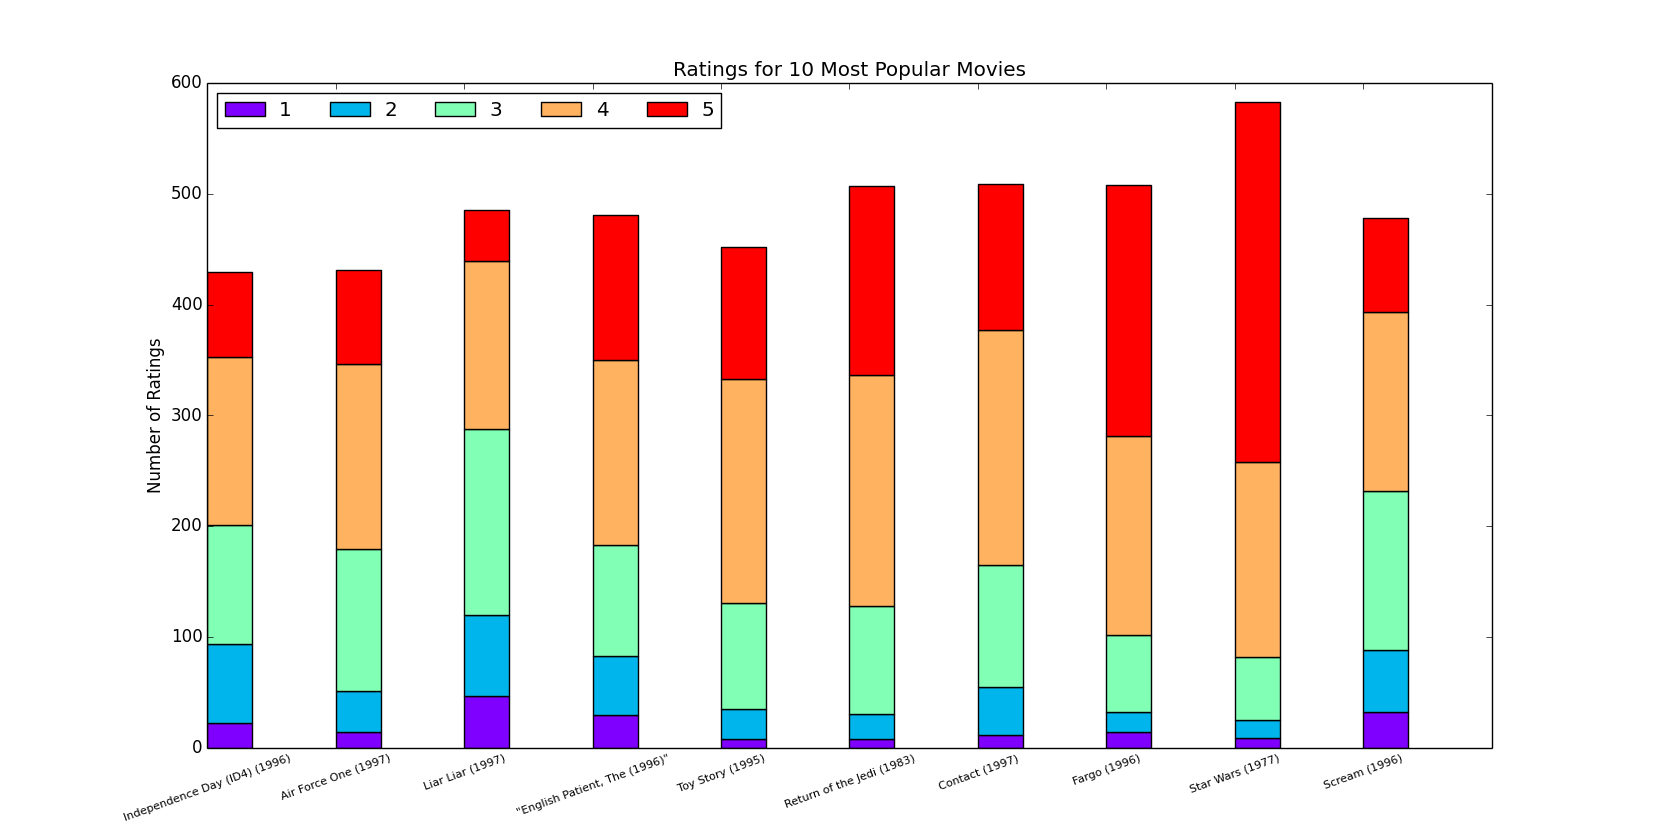
\includegraphics[width=\textwidth]{most-popular}
    \caption{Visualization of ratings for most popular movies in the dataset.}
    \end{figure}

    \pagebreak
    \item \boldline{All ratings of the ten best movies (movies with the highest average ratings).}

    \begin{figure}[H]
    \centering
    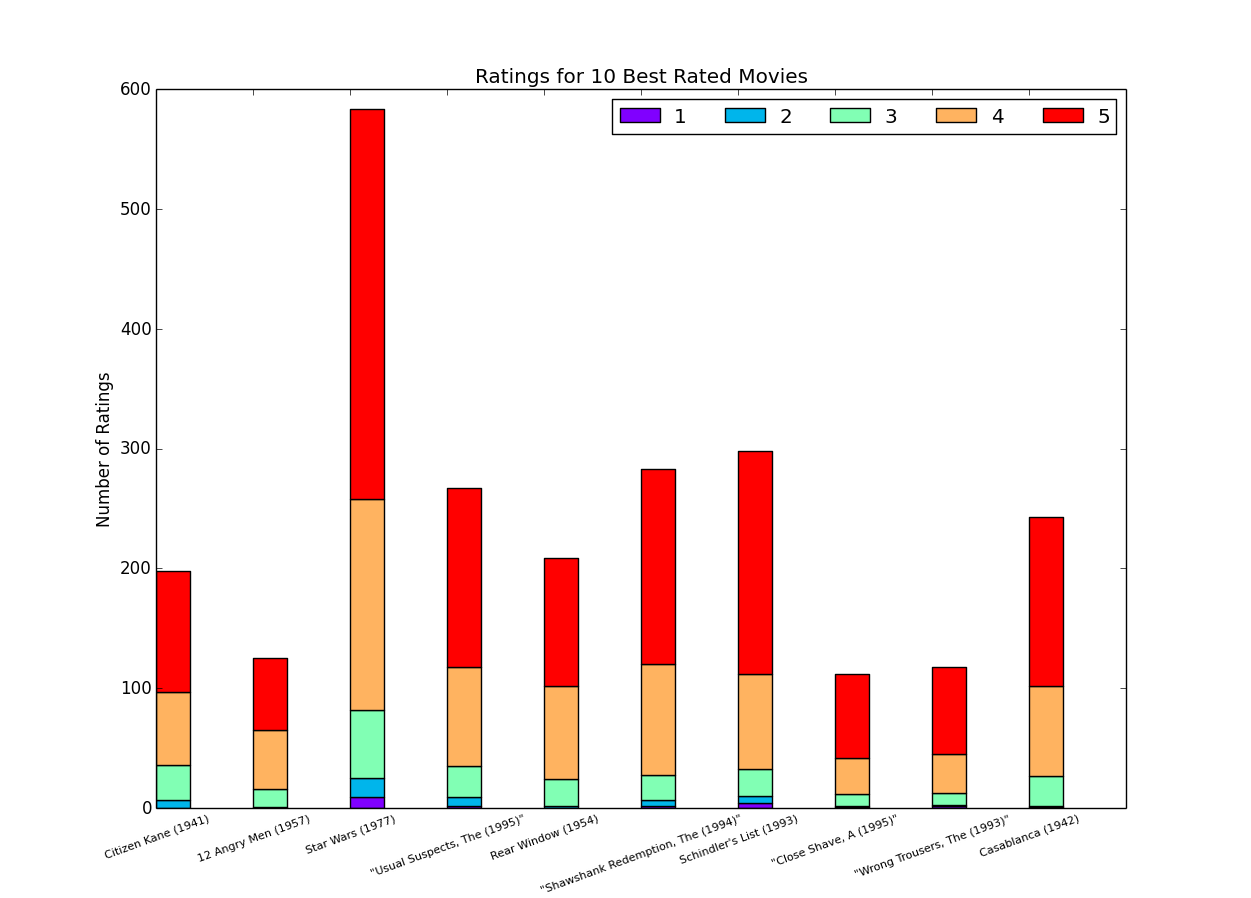
\includegraphics[width=\textwidth]{best-rated}
    \caption{Visualization of ratings for best rated movies in the dataset.}
    \end{figure}

    \pagebreak
    \item \boldline{All ratings of movies from the Crime genre.}

    \begin{figure}[H]
    \centering
    \includegraphics[width=\textwidth]{Crime_ratings_bar_chart}
    \caption{Visualization of ratings for all Crime movies in the dataset.}
    \end{figure}

    \pagebreak
    \item \boldline{All ratings of movies from the Documentary genre.}

    \begin{figure}[H]
    \centering
    \includegraphics[width=\textwidth]{Documentary_ratings_bar_chart}
    \caption{Visualization of ratings for all Documentary movies in the dataset.}
    \end{figure}


    \pagebreak
    \item \boldline{All ratings of movies from the Fantasy genre.}

    \begin{figure}[H]
    \centering
    \includegraphics[width=\textwidth]{Fantasy_ratings_bar_chart}
    \caption{Visualization of ratings for all Fantasy movies in the dataset.}
    \end{figure}











    \pagebreak
    \item \boldline{2D Visualization of 10 Random Movies}

    \begin{figure}[H]
    \centering
    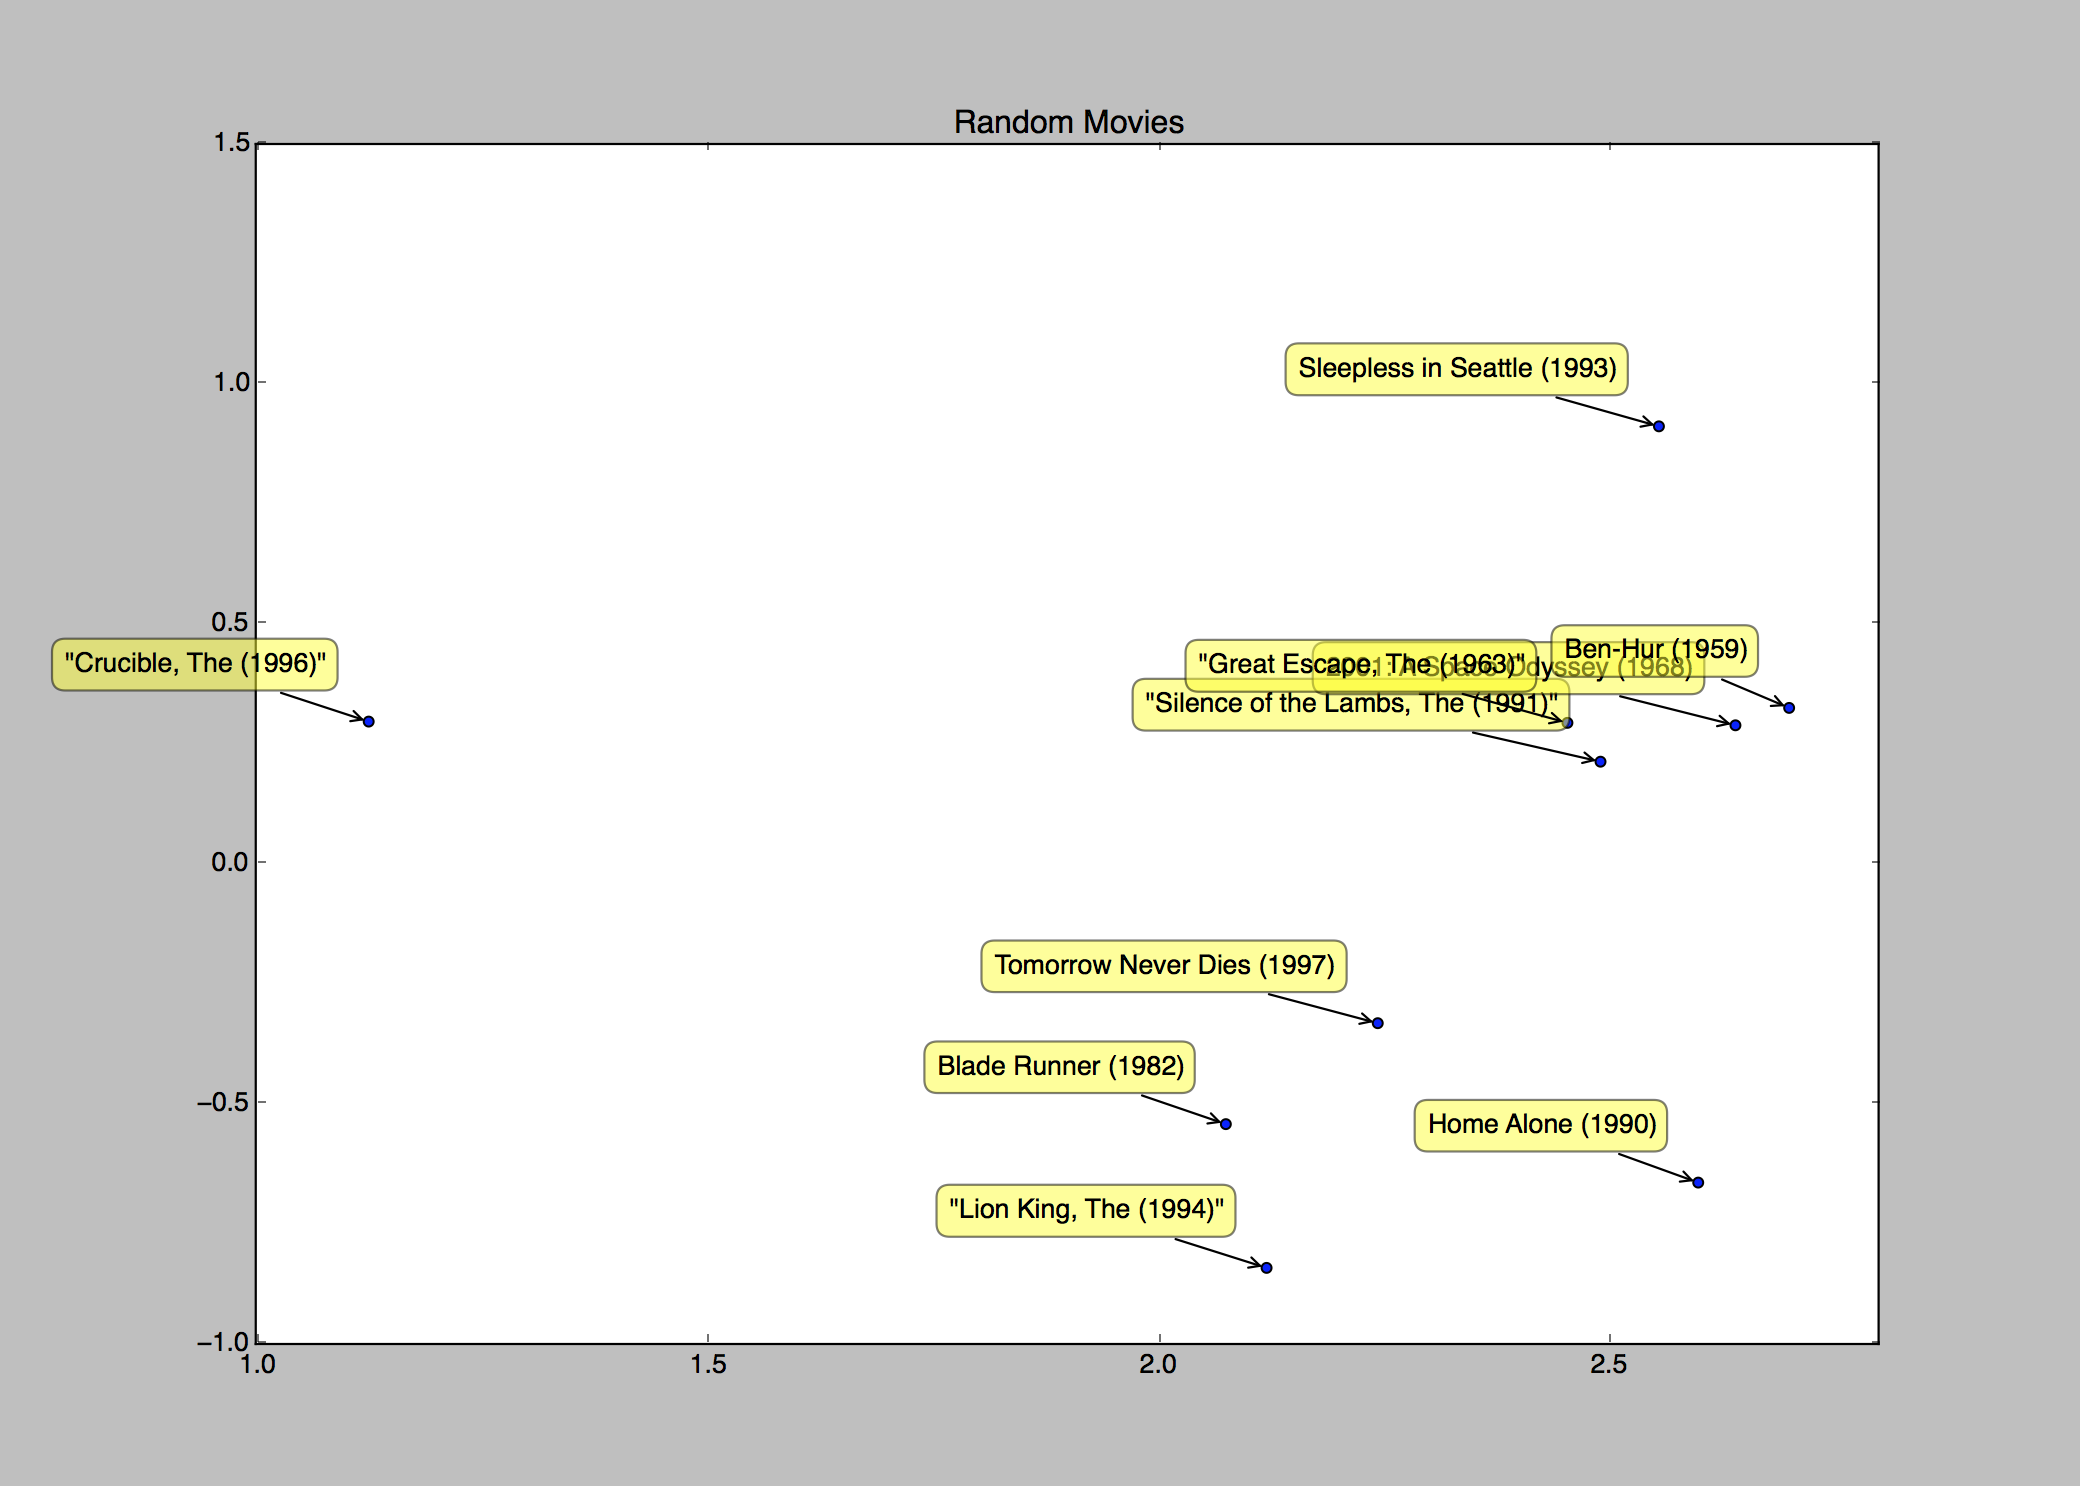
\includegraphics[width=\textwidth]{random_2d_vis}
    \caption{2D visualization of parameters for 10 random movies in the dataset.}
    \end{figure}


    \pagebreak
    \item \boldline{2D Visualization of 10 Most Popular Movies}

    \begin{figure}[H]
    \centering
    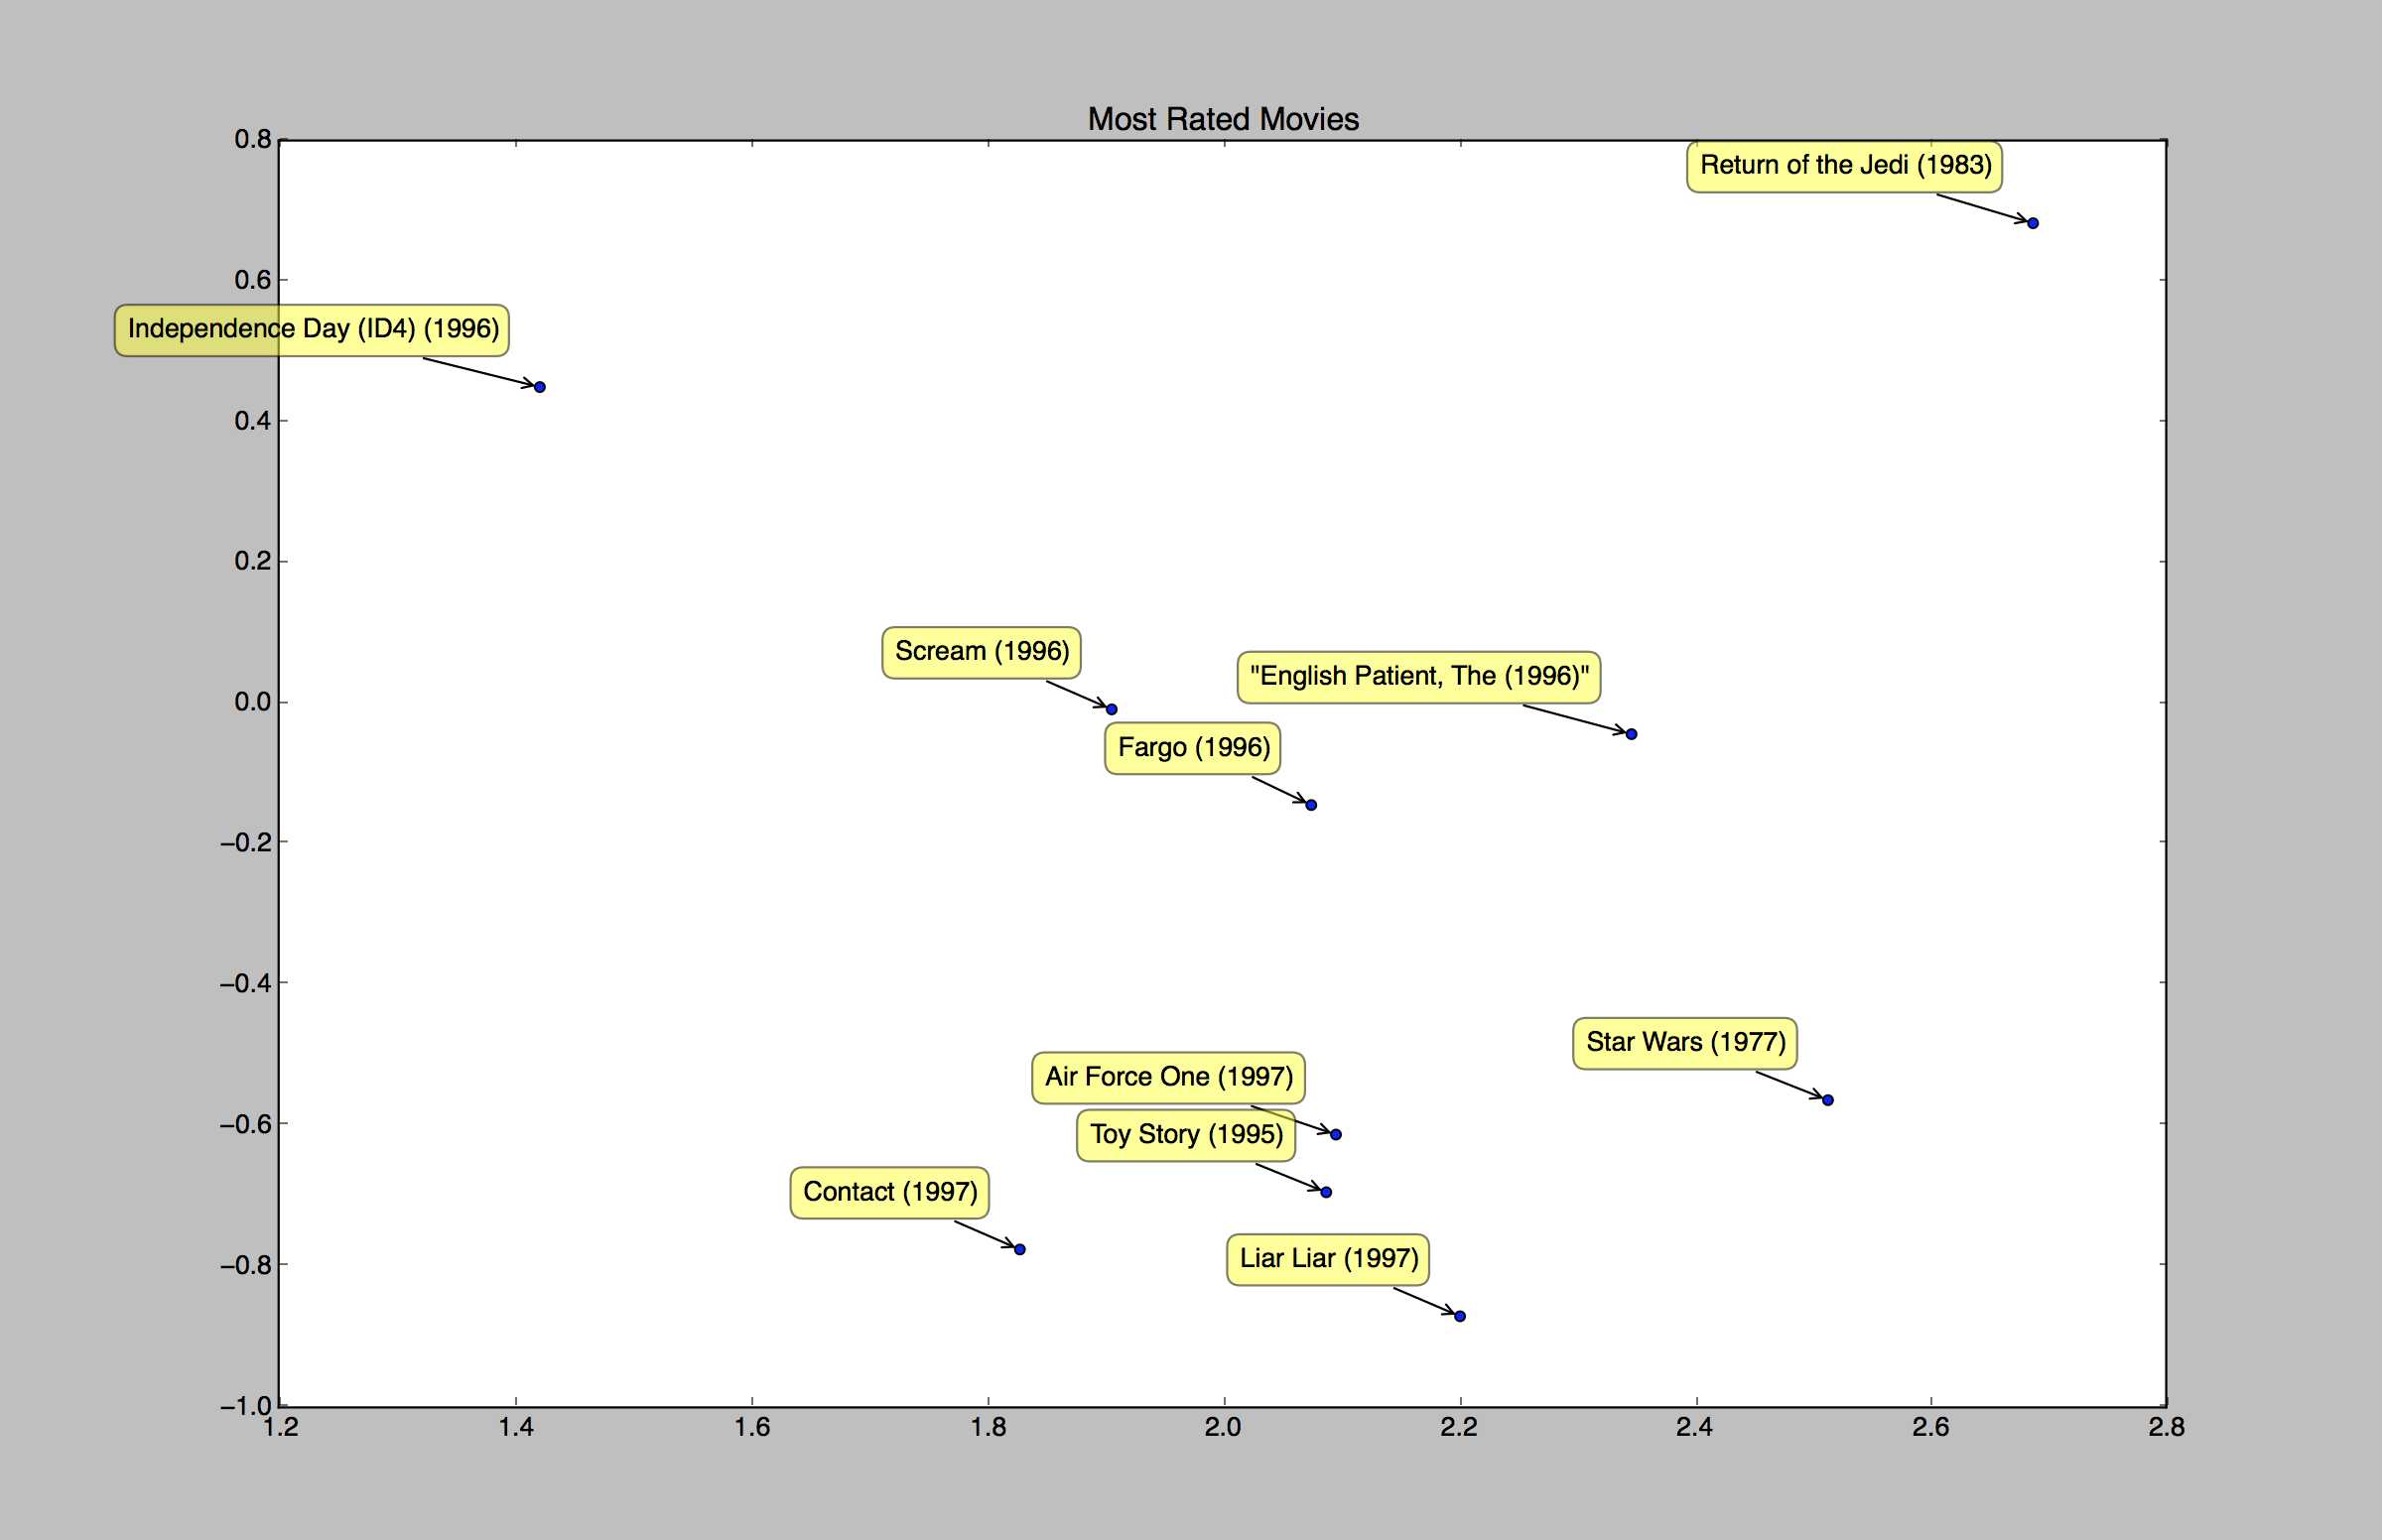
\includegraphics[width=\textwidth]{popular_2d_vis}
    \caption{2D visualization of parameters for 10 most popular movies in the dataset.}
    \end{figure}


    \pagebreak
    \item \boldline{2D Visualization of 10 Best Movies}

    \begin{figure}[H]
    \centering
    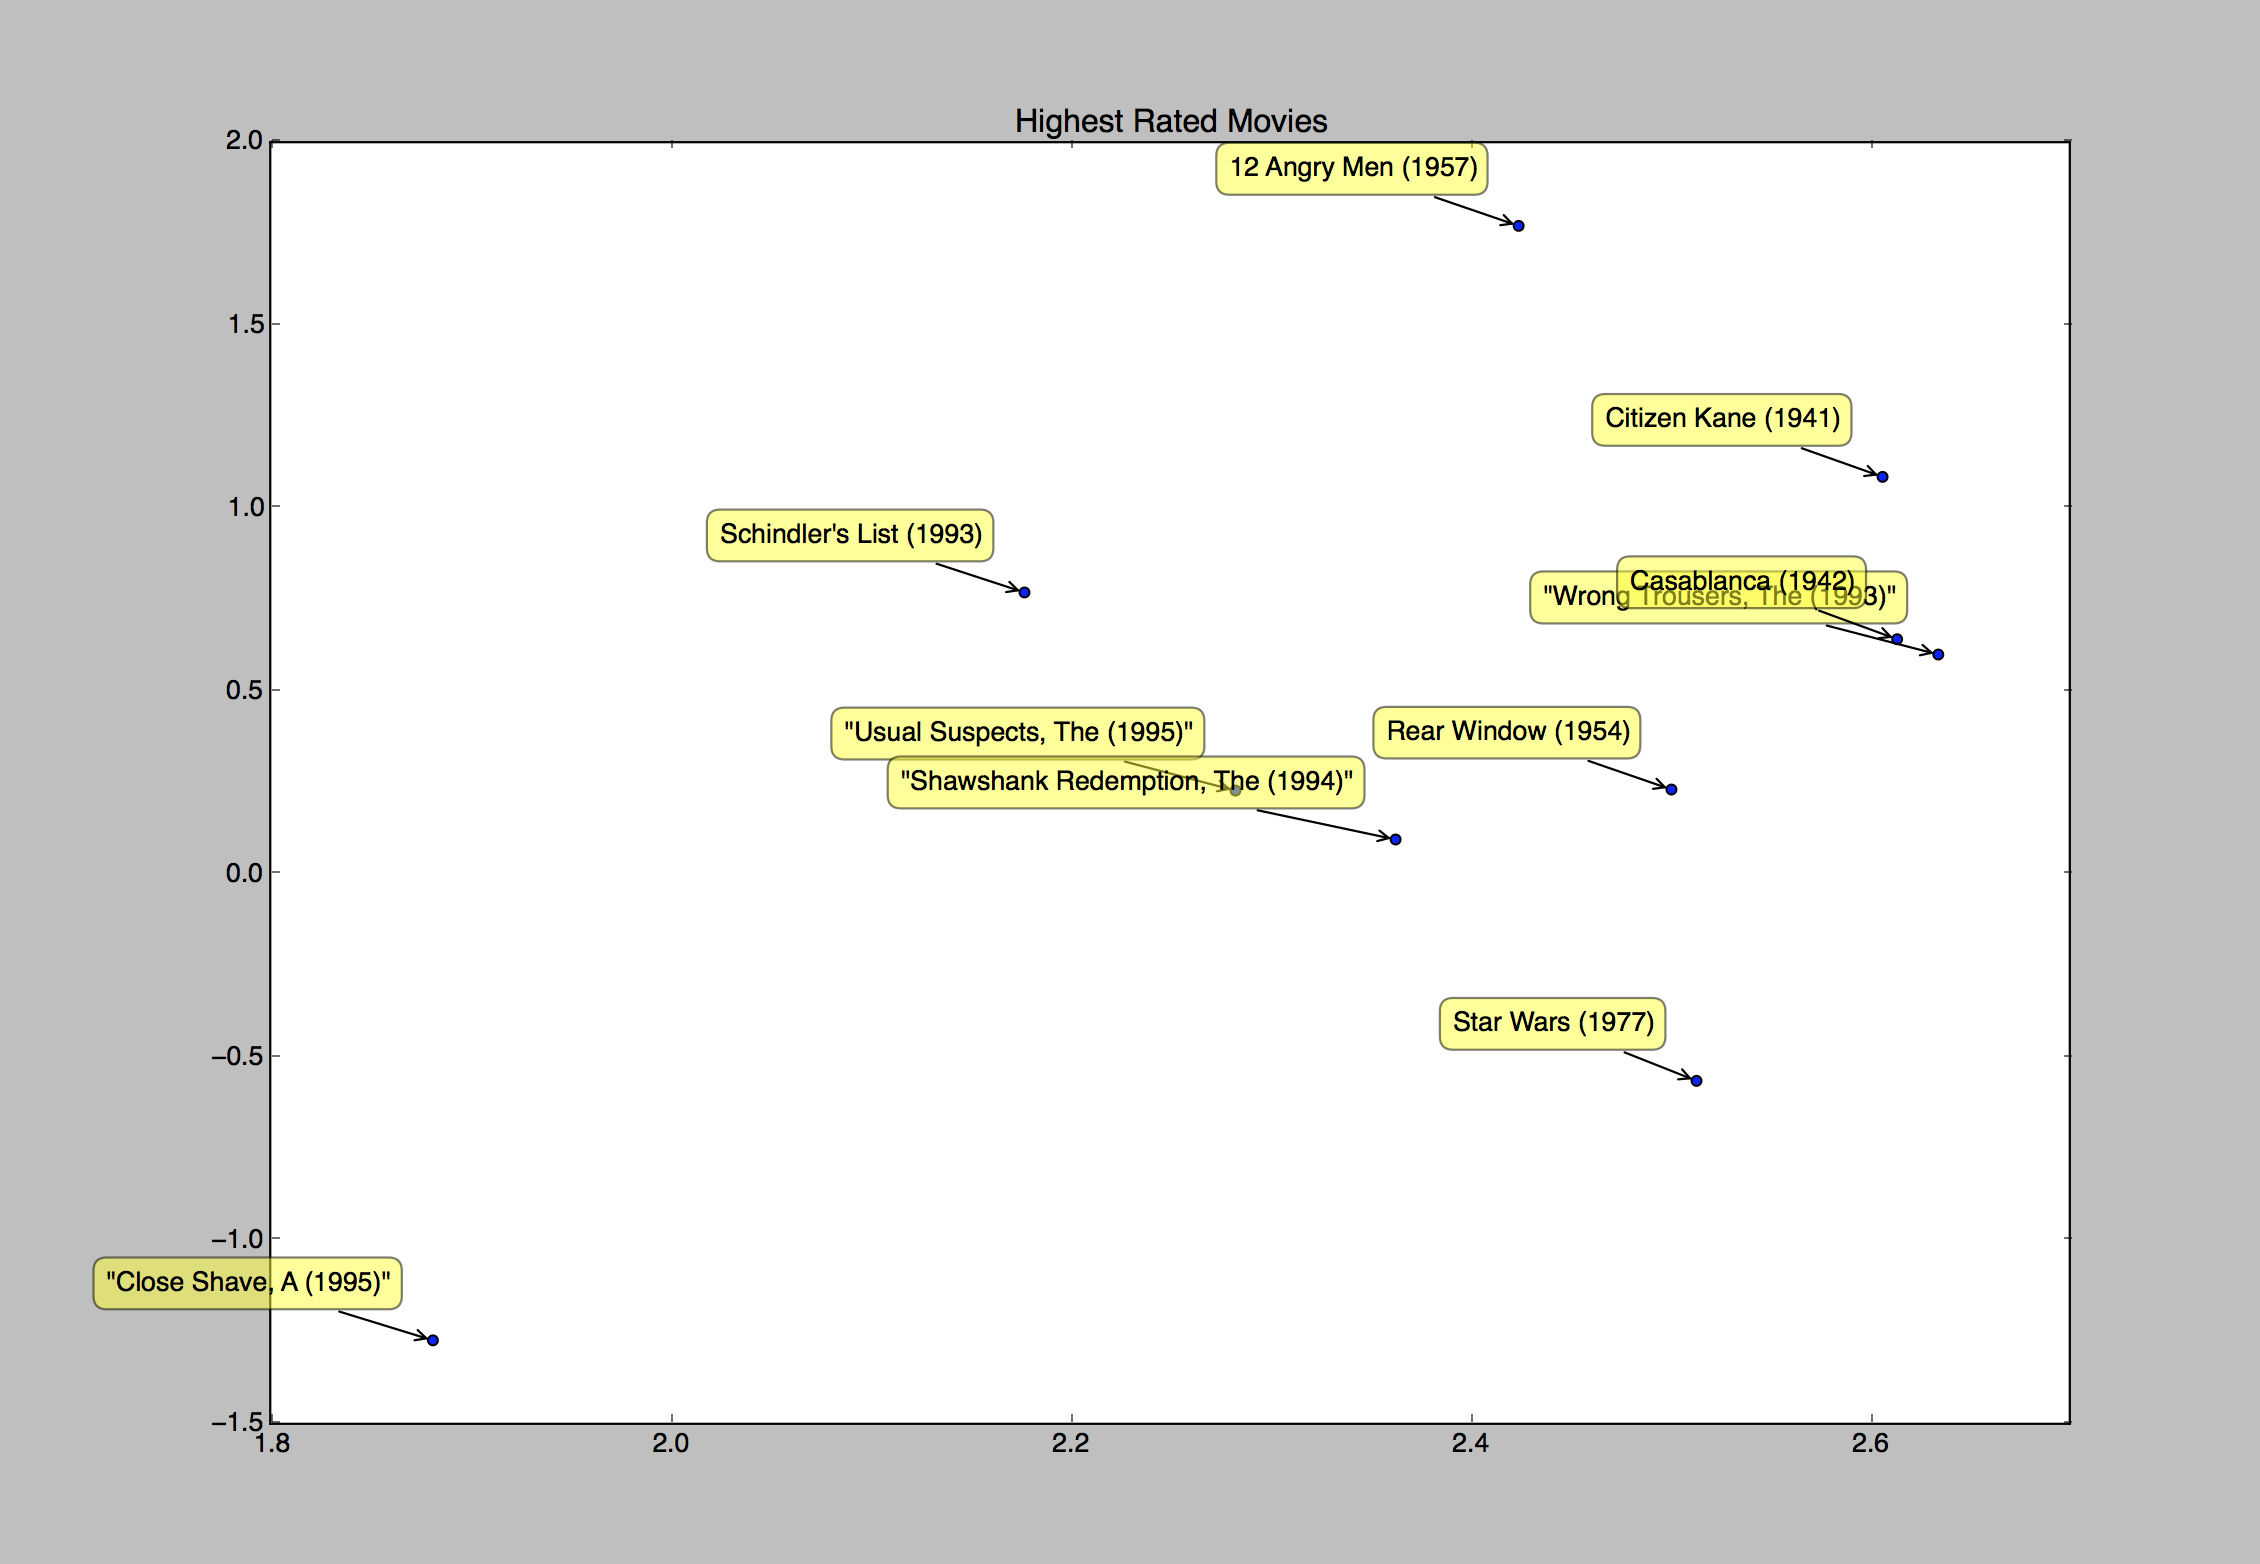
\includegraphics[width=\textwidth]{highest_2d_vis}
    \caption{2D visualization of parameters for 10 best movies in the dataset.}
    \end{figure}



    \pagebreak
    \item \boldline{2D Visualization of 10 Crime Movies}

    \begin{figure}[H]
    \centering
    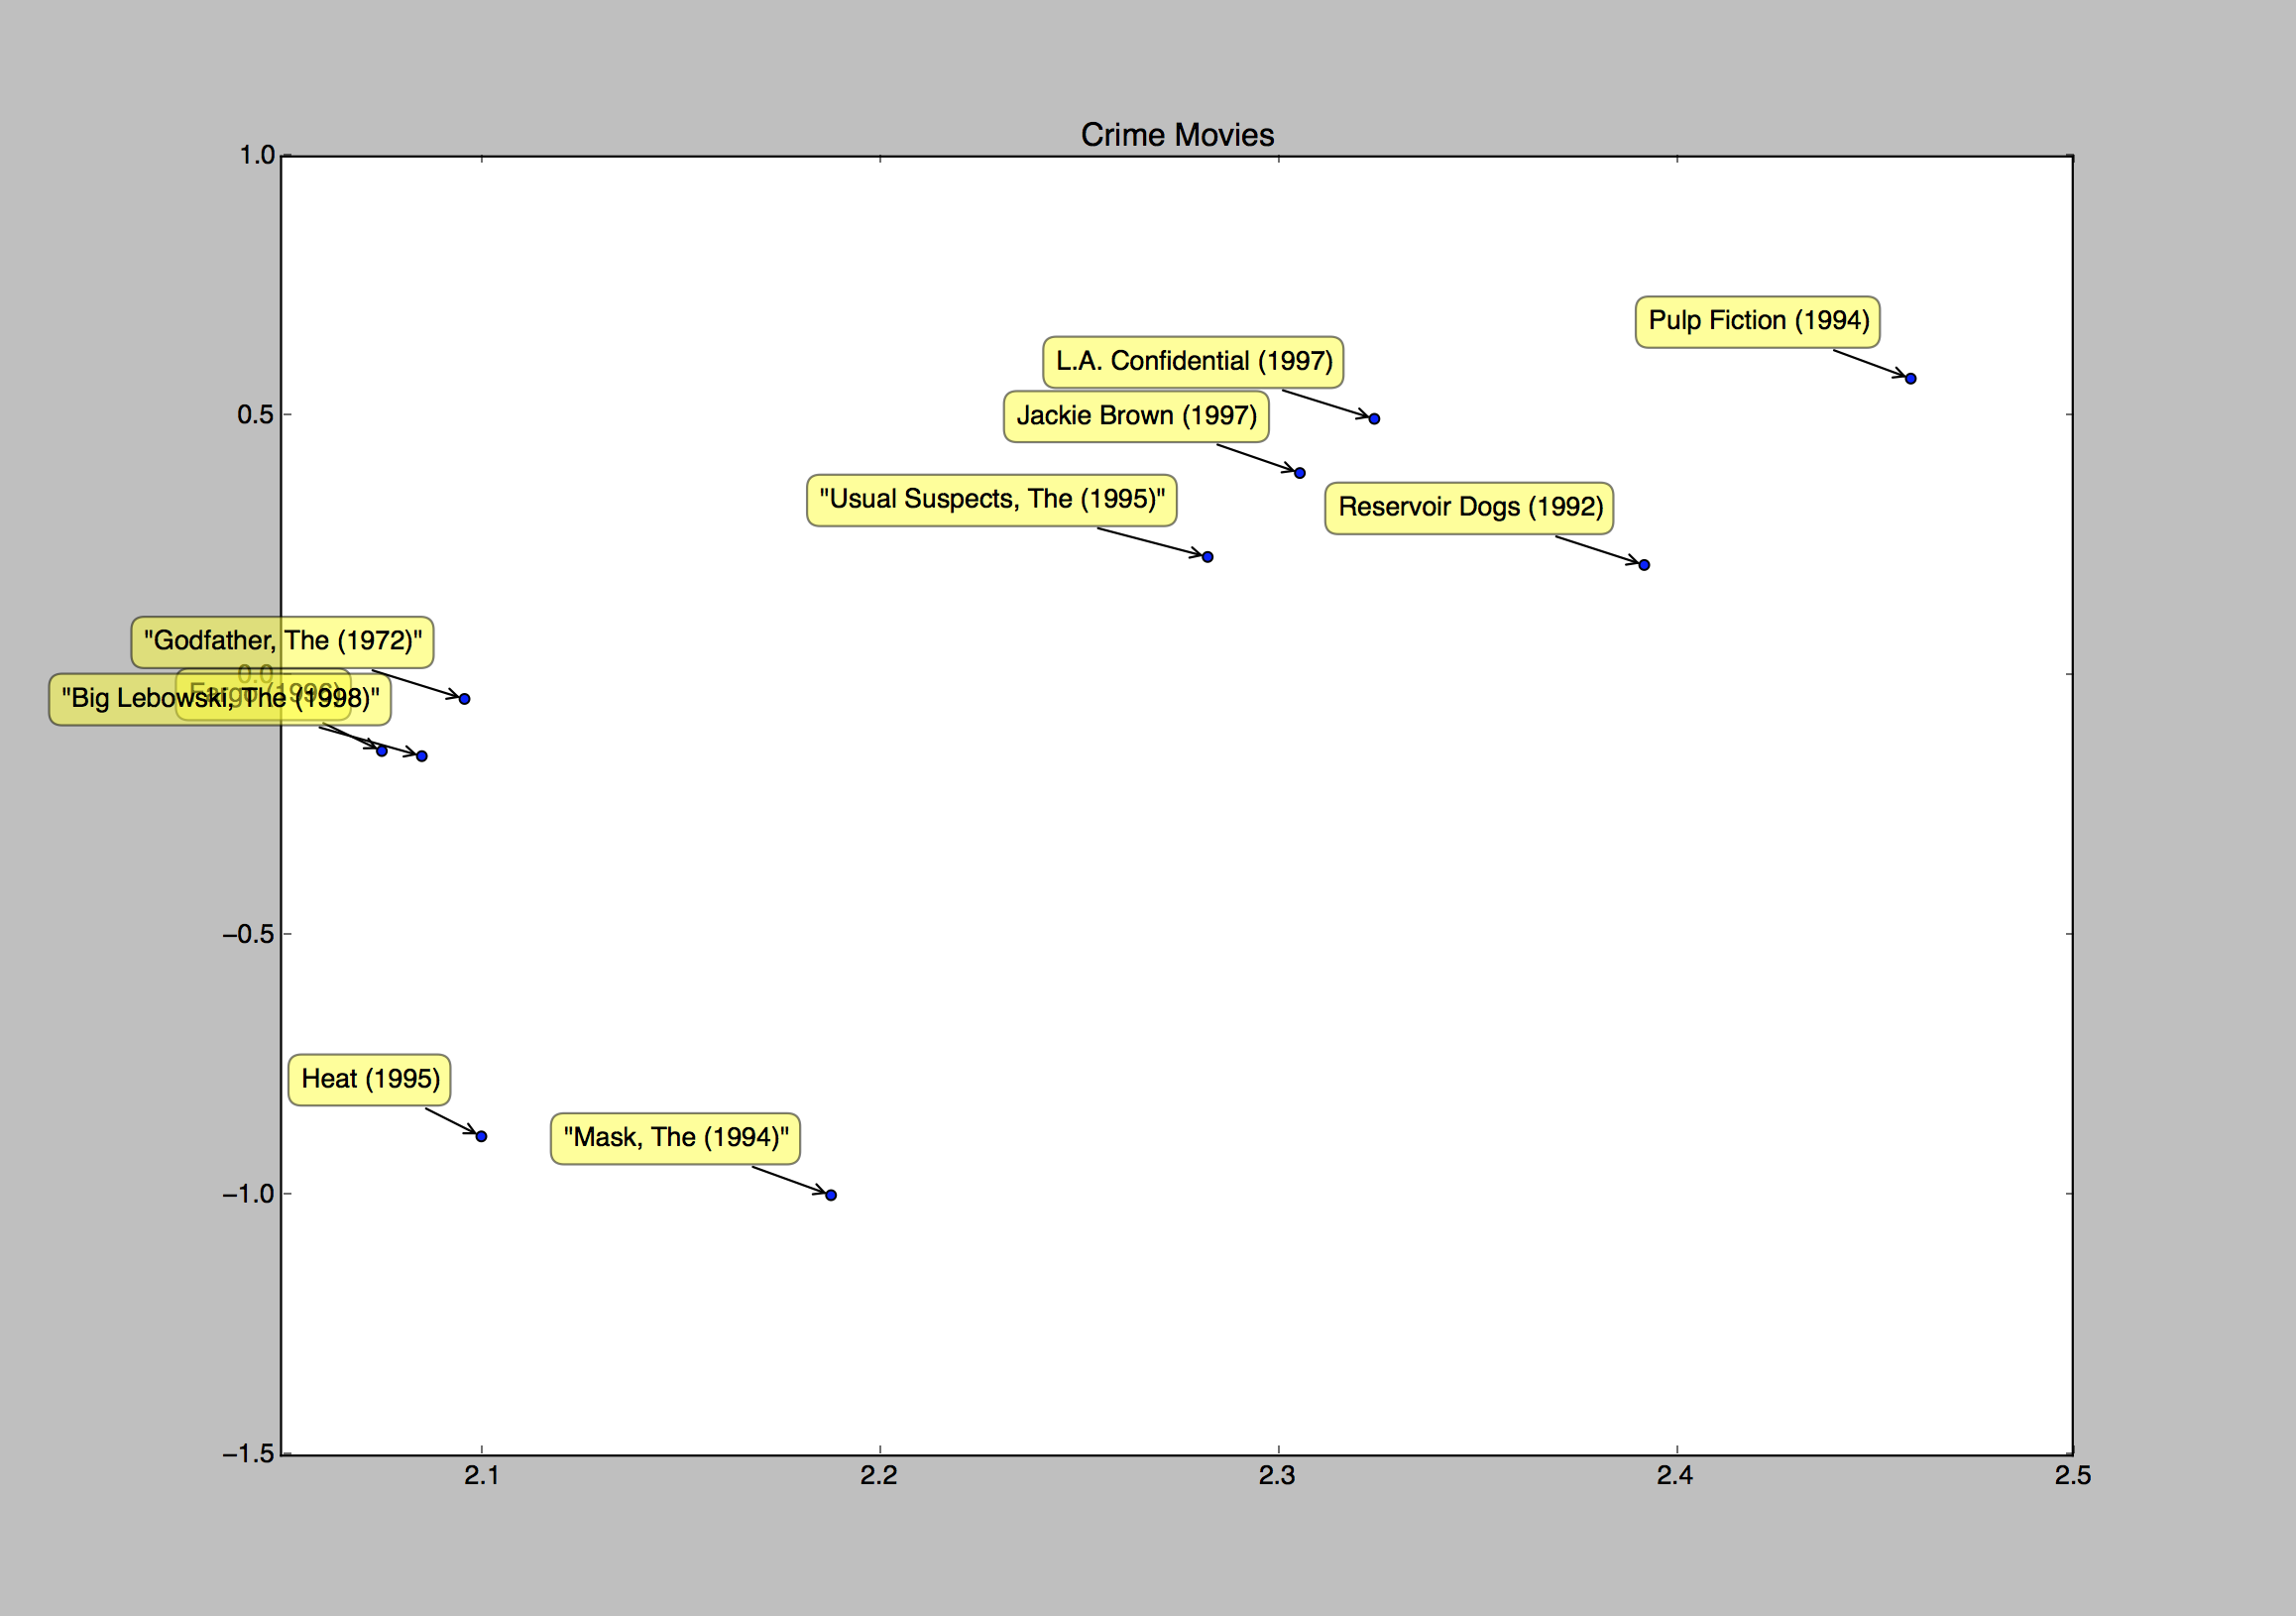
\includegraphics[width=\textwidth]{crime_2d_vis}
    \caption{2D visualization of parameters for 10 crime movies in the dataset.}
    \end{figure}


    \pagebreak
    \item \boldline{2D Visualization of 10 Documentary Movies}

    \begin{figure}[H]
    \centering
    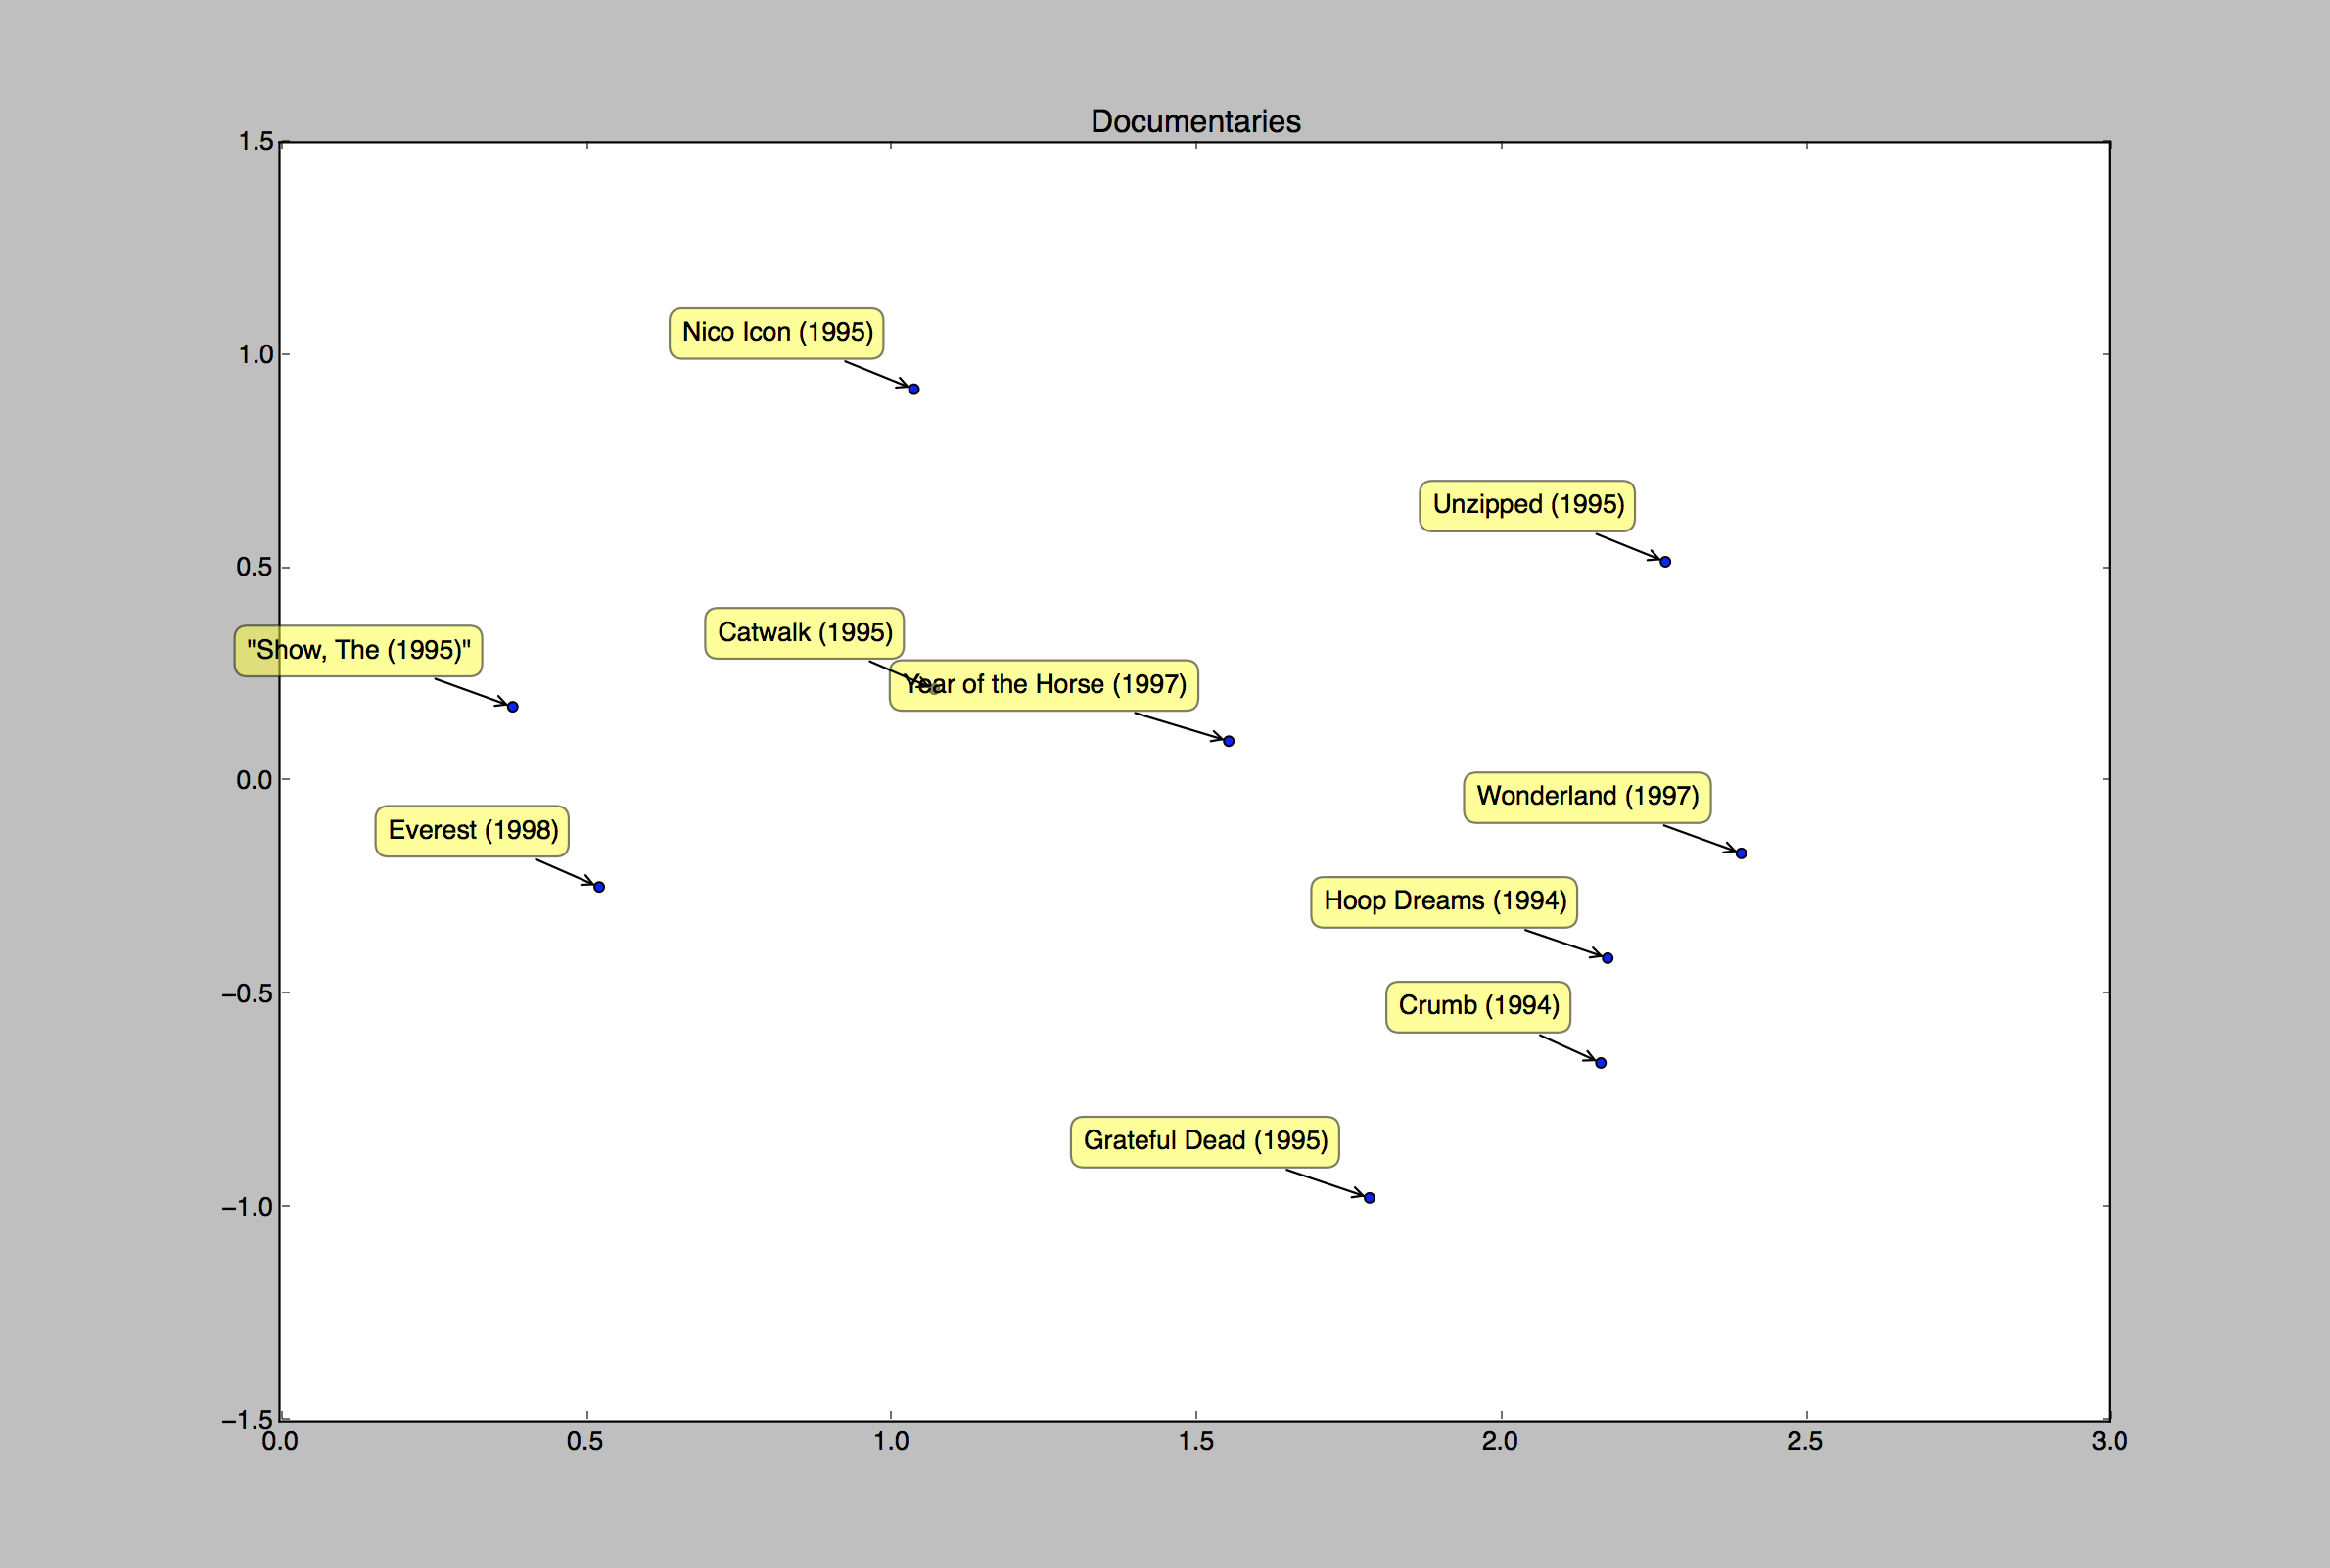
\includegraphics[width=\textwidth]{documentaries_2d_vis}
    \caption{2D visualization of parameters for 10 documentary movies in the dataset.}
    \end{figure}


    \pagebreak
    \item \boldline{2D Visualization of 10 Fantasy Movies}

    \begin{figure}[H]
    \centering
    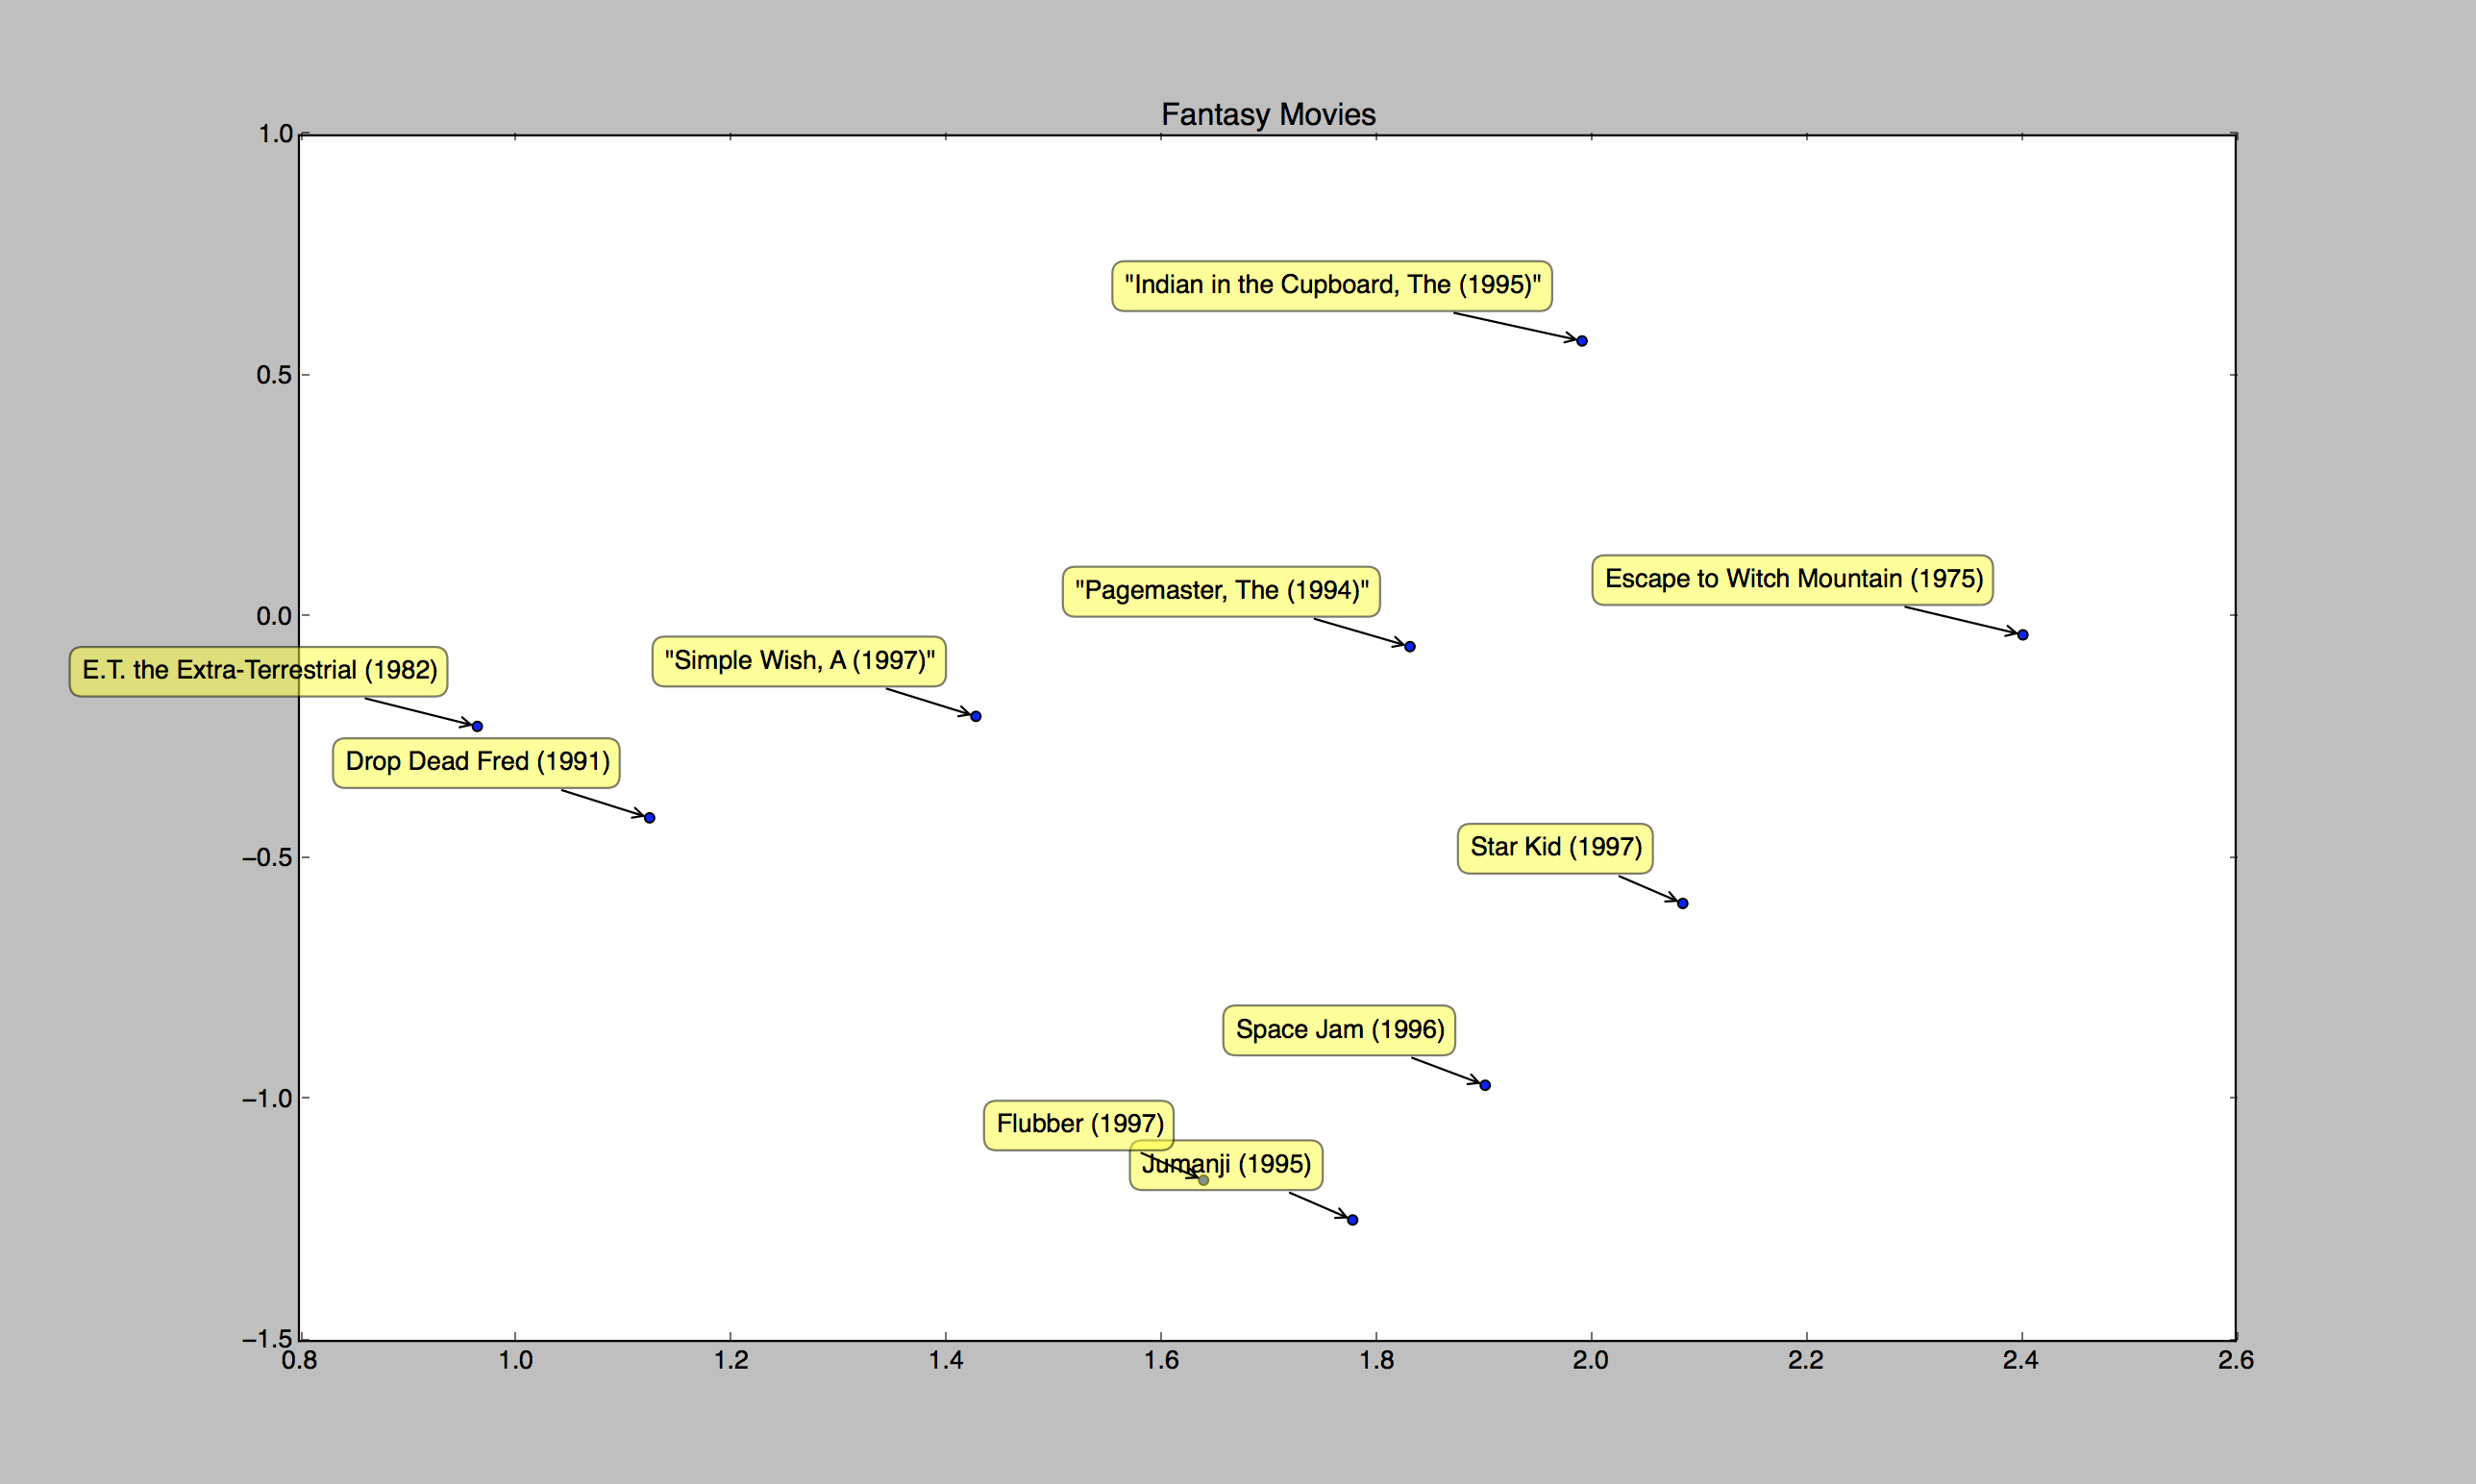
\includegraphics[width=\textwidth]{fantasy_2d_vis}
    \caption{2D visualization of parameters for 10 fantasy movies in the dataset.}
    \end{figure}




\end{itemize}






\end{document}
